\chapter{Introdução}

  A Organização das Nações Unidas (ONU) divulgou em 2015 o seu relatório referente
  às perspectivas de crescimento populacional, que constatou uma população mundial
  de 7,3 bilhões na metade do ano de 2015, projetando ainda, para 2030, um aumento
  para 8,5 bilhões \cite{ONU2015}. Esse aumento populacional representa também um
  aumento significativo na demanda por alimentos, energia e infraestrutura.
  A indústria agrícola tem um papel essencial ao satisfazer essa demanda por alimentos,
  de forma que o aumento de produtividade e eficiência é muito importante.

  A utilização de tecnologias para o aperfeiçoamento do processo produtivo e
  diminuição de custos já é há muito conhecida. Segundo \cite{RAMIZ1988},
  “os custos de produção podem variar por diversos motivos. Pode-se destacar a
  utilização intensiva ou não de tecnologia”. Uma das soluções propostas é a
  utilização de robôs automatizados (também conhecidos como rovers) para a
  análise do solo e de suas propriedades e necessidades, tornando customizado
  o uso de insumos para o processo produtivo.

  Estas tecnologias também podem melhorar os números em termos de sustentabilidade.
  O setor agrícola é o que mais consome e também o que mais desperdiça água doce no país.
  Aproximadamente 70\% da água utilizada no Brasil é destinada as suas atividades
  e quase metade desse valor é jogada fora. Entre os motivos do desperdício estão
  irrigações mal executadas e falta de controle do agricultor na quantidade usada
  em lavouras e no processamento dos produtos \cite{fao2013}.

  \section{Problemática}

  O desenvolvimento da agricultura através de métodos tradicionais vem se
  mostrando cada dia mais obsoleto, uma vez que não acompanha inovações
  tecnológicas \cite{ROCHA2015}. Essa transferência de tecnologia para aplicações
  práticas em processos produtivos muitas vezes ocorre de forma lenta, já que
  os produtores se mostram resistentes a alterações em um sistema que funciona
  relativamente bem. Entretanto, a não adoção dessas tecnologias acarreta
  prejuízos das mais diversas formas. Ao abdicar de uma análise detalhada do
  solo, um produtor agrícola gera custos desnecessários de irrigação, nutrição
  do solo, controle de acidez, além da inevitável queda na qualidade do produto
  final. Mesmo que exista uma análise laboratorial por amostragem, esse método
  não demonstra ser tão eficiente quanto uma análise automatizada, já que essa
  análise somente é feita em laboratórios específicos, podendo a amostra,
  durante o seu transporte, ter alterações em suas características, o que pode
  prejudicar o resultado final da análise. Uma produção baseada em inovações
  tecnológicas garante, portanto, o aumento de produtividade, diminuição de
  custos e reduz significativamente possíveis falhas humanas no diagnóstico de
  problemas.


  As causas para o problema, junto ao problema, foram representadas em um diagrama
  de causa e efeito, também conhecido como fishbone, conforme é possível ver
  na figura abaixo.

  \begin{figure}[h]
    \centering
    \label{fig01}
      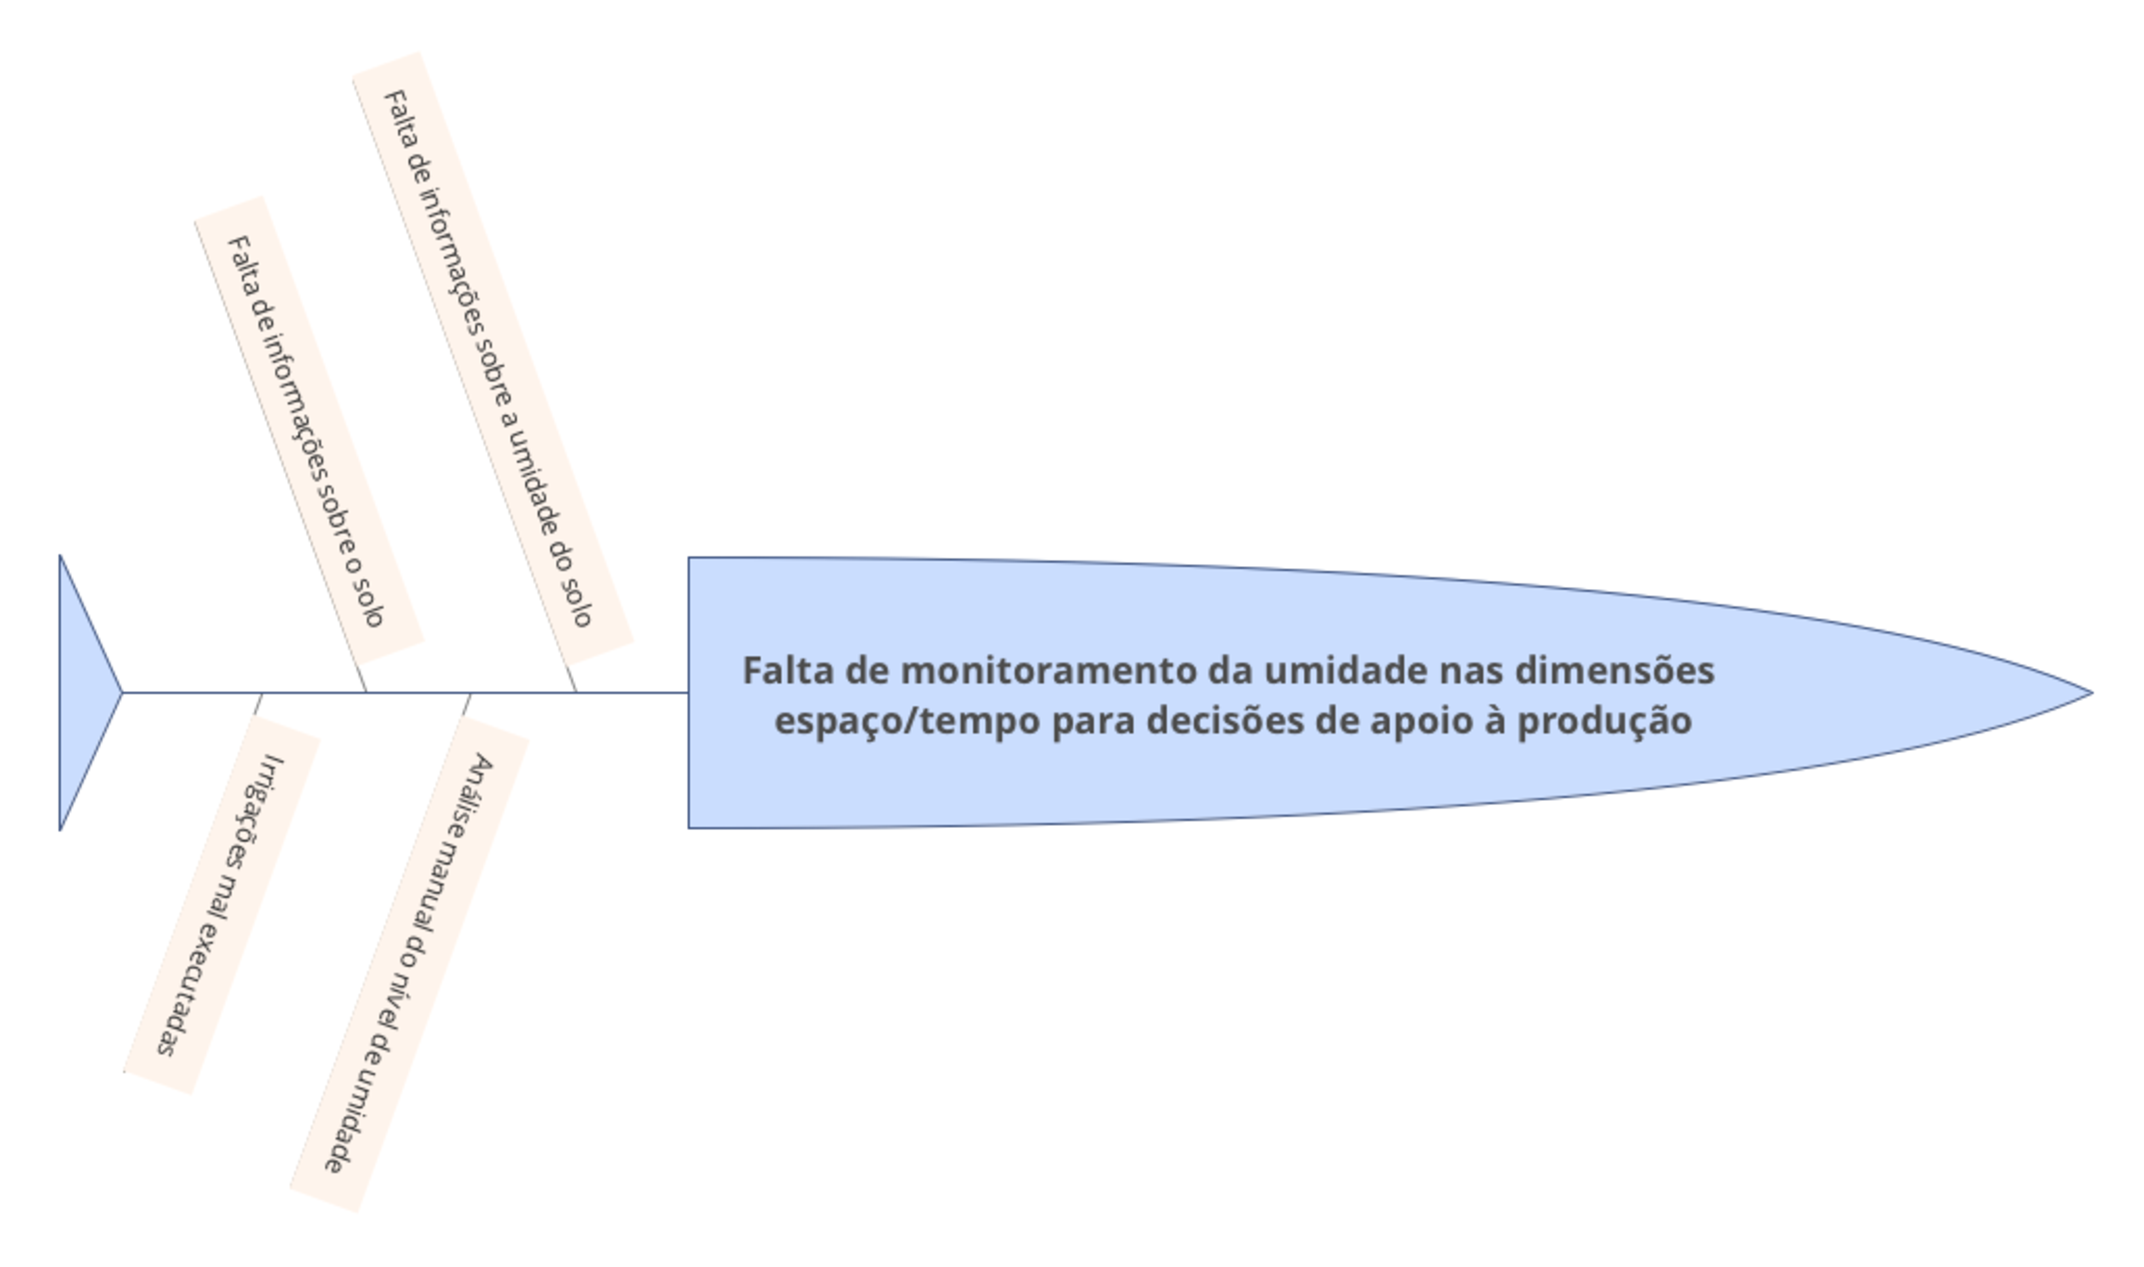
\includegraphics[keepaspectratio=true,scale=0.5]{figuras/fig01.eps}
    \caption{Diagrama de causa e efeito (\textit{fishbone}) para mapeamento do problema}
  \end{figure}

  Para uma descrição mais clara e formal do problema, foi utiliza o seguinte
  framework de descrição de problema:

  \textbf{O problema:} Falta de monitoramento da umidade nas dimensões espaço/tempo
  para decisões de apoio à produção.

  \textbf{Afeta:} Produtores de morangos.

  \textbf{Cujo impacto é:} Má irrigação das plantações, diminuição da qualidade
  do produto final e desperdício de água.

  \textbf{Uma solução bem sucedida seria:} A criação de um robô que automatiza
  a coleta da umidade em diversos pontos de uma lavoura.

  \vfill
  \pagebreak

  \section{Estado da Arte}

  Dentre as tecnologias existentes, protótipos como o rover, desenvolvido pela
  Embrapa em conjunto com a Universidade de São Paulo, e o “Robô Autônomo para
  Monitoramento do Solo” pela Universidade de Virgínia, se destacam como
  potenciais tecnologias no ramo da automatização agrícola e possuem grande
  potencial de inserção no mercado.  Entretanto estas tecnologias não são
  amplamente utilizadas no mercado por se tratarem de protótipos e não haver
  produção em massa consolidada.

  O rover desenvolvido pela EMBRAPA utiliza uma tecnologia de análise óptica
  para adquirir dados do solo. Essa tecnlogia se chama LIBS (Espectroscopia de
  emissão óptica com plasma induzido por laser), onde um laser de alta energia
  é focalizado sobre o solo, fazendo com que seja formado um plasma.
  Esse plasma realiza uma análise multielementar do solo \cite{ARCHILA2014}.

  \begin{figure}[h]
    \centering
    \label{fig01}
      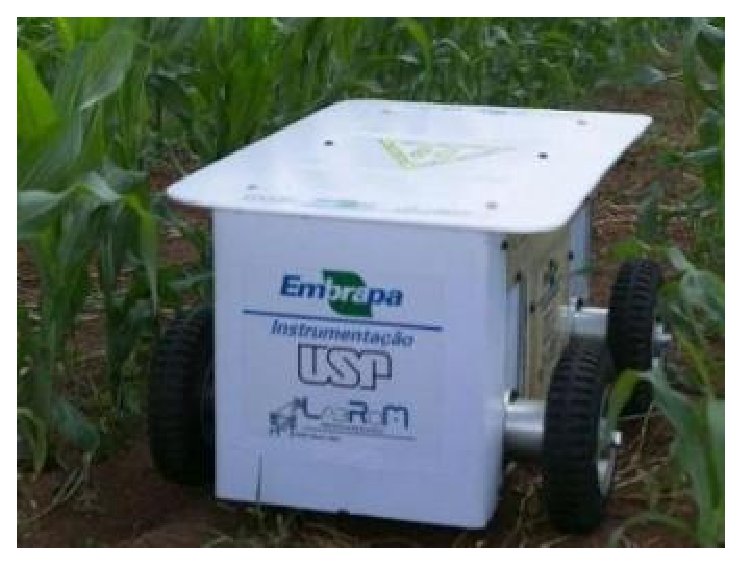
\includegraphics[keepaspectratio=true,scale=0.5]{figuras/fig02.eps}
    \caption{Rover desenvolvido pela EMPRAPA com tecnologia LIBS. Fonte: \cite{ARCHILA2014}}
  \end{figure}

  Este rover utiliza dois motores de corrente direta (DC) BTS7960 Arduino, três
  baterias de 12 Volts e 7 Ampére-hora, um conversor 3,3-5 Volts, e a arquitetura
  é formada por um microcontrolador Raspberry-pi, encarregado de enviar sinais
  de controle para o sistema de propulsão, além de ter os motores ligados a um
  Arduino UNO, encarregado de gerar sinais de PWM (Pulse-width modulation),
  controlando assim o sentido de giro dos motores e suas velocidades \cite{ARGOTE2014}.

  \section{Justificativa}

  Um sistema de monitoramento da umidade do solo envolve o desenvolvimento de
  técnicas de medição específicas para cada cenário de plantio. Esse tipo de
  monitoramento, além de reduzir custos com desperdício de recursos hídricos,
  podem melhorar significativamente as condições de plantio provendo um aumento
  nos níveis de produtividade e consequentemente uma melhora na qualidade do
  produto final.

  Algumas soluções foram encontradas e estudadas, a exemplo do projeto
  desenvolvido pela EMBRAPA, que utiliza tecnologia de laser LBS, mas que deixa
  a desejar em aspectos de viabilidade financeira e comercial. Visto que não
  foram encontradas soluções desenvolvidas a nível de mercado com as mesmas
  características do projeto proposto, esse trabalho tem o objetivo de atacar
  de maneira viável a operação e controle de umidade em uma lavoura de morangos
  através de um dispositivo relativamente barato e eficiente no que tange a seus
  objetivos operacionais e benefícios para a produção agropecuária.

  Após a validação de requisitos, análise do tempo disponível, custos e propostas
  de soluções, foi possível concluir que o projeto é viável, tanto de um ponto
  de vista técnico.

  \section{Objetivos}

  \subsection{Geral}

  O projeto possui como objetivo construir um veículo terrestre autônomo que,
  a partir de sensores apropriados, possa aferir os valores de umidade do solo,
  ar e temperatura do ar em uma plantação de morangos para que seja realizado
  um controle adequado em tais parâmetros.

  \subsection{Específicos}

  \begin{itemize}
    \item Analisar e dimensionar os componentes do veículo;
    \item Identificar meio de locomoção para o ambiente;
    \item Escolher técnica de medição adequada para as variáveis impactantes (umidade do solo e ar e temperatura do ar);
    \item Desenvolver sistema de localização para autonomia do veículo;
    \item Criar uma plataforma para a apresentação dos dados coletados.
  \end{itemize}

  \vfill
  \pagebreak

  \section{Escopo}

  A partir do problema identificado e dos objetivos elucidados pelo grupo,
  definiu-se o escopo geral do projeto. Para a validação da proposta, será feito
  o desenvolvimento do produto mínimo viável, que será aplicado como forma de
  estudo e solução para problemática envolvida neste trabalho. O produto mínimo
  contempla então, para fins de prototipação, as seguintes características:

  \begin{itemize}
    \item Um veículo capaz de se locomover em terreno areno-argiloso plano;
    \item Um veículo capaz de se locomover dentro da trilha de espaçamento de uma lavoura de morangos;
    \item Um veículo capaz de realizar um percurso completo pela lavoura, transitando pelos espaços entre as fileiras plantadas.
    \item Um veículo capaz de efetuar diversas medições da umidade do solo sob a planta em intervalos de distância predefinidos
    \item Um veículo capaz de  efetuar diversas medições da temperatura e umidade do ar em intervalos de distância predefinidos
    \item Um veículo capaz de armazenar os dados das medições em uma memória de fácil extração e acesso;
    \item Um sistema capaz de receber os dados em um arquivo e disponibilizar de forma gráfica;
    \item Um sistema capaz de gerar e exportar relatórios dos dados armazenados;
  \end{itemize}
